\documentclass{article}
\usepackage[T1]{fontenc} % Fontes T1
\usepackage[utf8]{inputenc} % Input UTF8
\usepackage[backend=biber, style=ieee]{biblatex} % para usar bibliografia
\usepackage{csquotes}
\usepackage[portuguese]{babel} %Usar língua portuguesa
\usepackage{blindtext} % Gerar texto automaticamente
\usepackage[printonlyused]{acronym}
\usepackage{hyperref} % para autoref
\usepackage{graphicx}
\usepackage{indentfirst}
\usepackage{float}
%\usepackage{amsmath, amssymb}
%\usepackage{caption}
%\usepackage{geometry}
\usepackage{array}
\usepackage{multirow}

%\usepackage{titlesec}

\usepackage{fancyhdr}

\pagestyle{fancy}  % Ativa o estilo fancyhdr

\lhead{
\includegraphics[width=0.5cm]{images/ua.pdf} UA}   % Cabeçalho à esquerda
\chead{Redes de Comunicações I}    % Cabeçalho no centro
\rhead{Grupo 4}    % Cabeçalho à direita

% Formato e espaçamento para os capítulos
%\titleformat{\chapter}[hang]{\huge\bfseries}{\thechapter}{10pt}{\Huge}
%\titlespacing*{\chapter}{0pt}{-20pt}{20pt} 


\bibliography{bibliografia}

\begin{document}
%%
% Definições
%
\def\titulo{Bobinas de Helmholtz}
\def\autores{Fábio Franco, João Marques, Ricardo Domingues}
\def\empresa{Universidade de Aveiro}
\def\logotipo{ua.pdf}
%
%%%%%% CAPA %%%%%%
%
\begin{titlepage}
    \centering
    {\LARGE {Redes de Comunicações I}}\\
    \vspace{0.5cm}
    {\LARGE Universidade de Aveiro}\\
    \vspace{1.5cm}
    
\includegraphics[width=1.5cm]{images/ua.pdf} % Adicione o logo da universidade se necessário
    \vspace{1.5cm}
    
    {\Large \textbf{Departamento de Eletrónica, Telecomunicações e Informática}}\\
    \vspace{0.5cm}
    {\large \textbf{Ano 2024/2025}}\\
    
    \vfill
    
    {\Large \textbf{Report - Fase 1}}\\
    \vspace{0.5cm}
    % \Large \textbf{Fase 1}}\\
    
    \vfill
    
    \vspace{2cm}
    \begin{center}
      \large \textbf{14 de Novembro de 2024}
    \end{center}
    \vspace{0.1cm}
    \begin{center}
    \fbox{\parbox{6cm}{\centering \textbf{P4 - Grupo 4}  \vspace{0.2cm} \\ Fábio Franco (119826) \vspace{0.1cm} \\ Ricardo Domingues (119521) \vspace{0.1cm} }}
    \end{center}
    
\end{titlepage}

\pagenumbering{roman}

%\renewcommand{\contentsname}{Índice}
%\tableofcontents
% \listoftables     % descomentar se necessário
% \listoffigures    % descomentar se necessário

%%%%%%%%%%%%%%%%%%%%%%%%%%%%%%%
\clearpage
\pagenumbering{arabic}

%%%%%%%%%%%%%%%%%%%%%%%%%%%%%%%%
%\chapter{Números Mecanográficos}
\vspace{1.0cm}
\section*{\centerline{Números Mecanográficos}}
Os números mecanográficos utilizados ao longo do projeto são 119826 e 119521, sendo:
\begin{itemize}
    \item $x_1$ -> 1
    \item $x_2$ -> 9
    \item $x_3$ -> 8
    \item $x_4$ -> 2
    \item $x_5$ -> 6
    \item $x_6$ -> 1
    \item $x_7$ -> 9
    \item $x_8$ -> 5
    \item $x_9$ -> 2
    \item $x_{10}$ -> 1
\end{itemize}

\vspace{0.2cm}
Endereços IP utilizados ao longo do projeto:

\begin{table}[h!]
\centering
\begin{tabular}{|c|c|c|}
    \hline
     & \textbf{Calendar Inc} & \textbf{Horoscope Inc} \\ \hline
    \textbf{Public IPv4(sub) Network} & 203.128.191.128/25 & 203.012.059.0/25 \\ \hline
    \textbf{Private IPv4 Network} & 172.26.012.0/23 & 172.22.012.0/23 \\ \hline
    \textbf{Global IPv4 Network} & 2002:A198:BC26::/48 & 2002:A125:BC91::/48 \\ \hline
\end{tabular}
\caption{Endereços IP utilizados}
\label{tab:exemplo}
\end{table}

\newpage
%\clearpage

\section*{\centerline{Public IPv4}}
%\chapter{Public IPv4}
\vspace{0.5cm}
\subsection*{Calendar Inc}

\begin{table}[h!]
\hspace*{-3.0cm}
\centering
%\begin{tabular}{|m{2cm}|m{1,3cm}|m{2,3cm}|m{5cm}|m{2,5cm}|m{1cm}|}
\begin{tabular}{|c|c|c|c|c|c|}
    \hline
    & \textbf{Máscara} & \textbf{Rede} & \textbf{Endereços Disponíveis} & \textbf{Broadcast} & \textbf{Default Gateway} \\ \hline
    NAT/PAT & 30 & 203.128.191.184 & 203.128.191.185 a 203.128.191.187 & --- & --- \\ \hline
    VLAN2 & 28 & 203.128.191.160 & 203.128.191.162 a 203.128.191.174 & 203.128.191.175 & 203.128.191.161\\ \hline
    VLAN4 & 27 & 203.128.191.128 & 203.128.191.130 a 203.128.191.158 & 203.128.191.159 & 203.128.191.129\\ \hline
    VLAN6 & 26 & 203.128.191.192 & 203.128.191.194 a 203.128.191.254 & 203.128.191.255 & 203.128.191.193\\ \hline
    VLAN8 & 29 & 203.128.191.176 & 203.128.191.178 a 203.128.191.182 & 203.128.191.183 & 203.128.191.177\\ \hline
    VLAN12 & 30 & 203.128.191.188 & 203.128.191.190 & 203.128.191.191 & 203.128.191.189\\ \hline
\end{tabular}
\caption{Atribuição do IPv4 Público para Calendar Inc}
\label{tab:exemplo5x6}
\end{table}

\begin{figure}[H]
    \hspace*{-1.5cm}
    \centering
    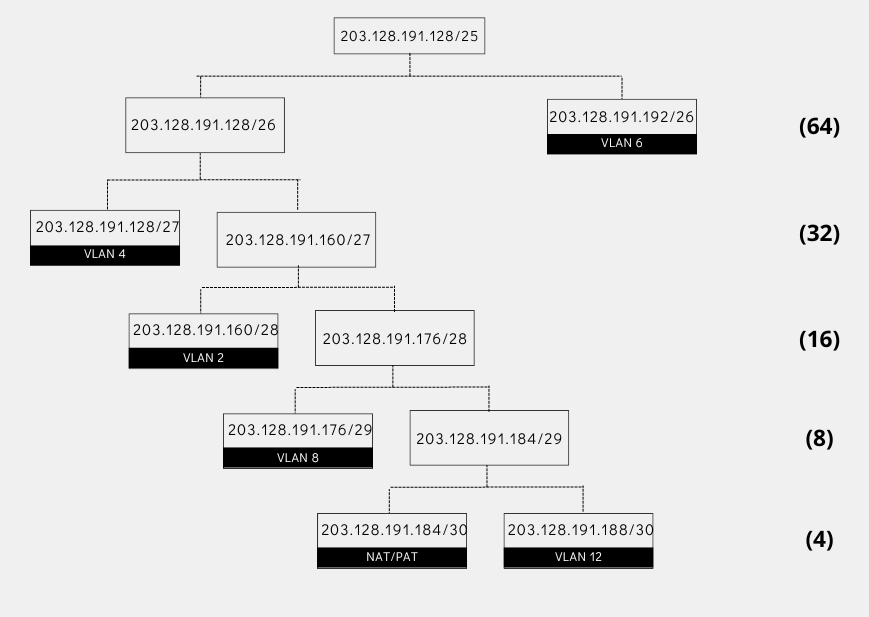
\includegraphics[width=15cm]{images/CalendarInc-IPv4 Publico.png}
   % \caption{Legenda da imagem, se desejar} % Opcional
\end{figure}
\newpage
\clearpage
\section*{Horoscope Inc}

\begin{table}[h!]
\hspace*{-2.0cm}
\centering
%\begin{tabular}{|m{2cm}|m{1,3cm}|m{2,3cm}|m{5cm}|m{2,5cm}|m{1cm}|}
\begin{tabular}{|c|c|c|c|c|c|}
    \hline
    & \textbf{Máscara} & \textbf{Rede} & \textbf{Endereços Disponíveis} & \textbf{Broadcast} & \textbf{Default Gateway} \\ \hline
    NAT/PAT & 30 & 203.12.59.56 & 203.12.59.57 a 203.12.59.59 & --- & --- \\ \hline
    VLAN14 & 27 & 203.12.59.0 & 203.12.59.2 a 203.12.59.30 & 203.12.59.31 & 203.12.59.1\\ \hline
    VLAN16 & 27 & 203.12.59.96 & 203.12.59.98 a 203.12.59.126 & 203.12.59.127 & 203.12.59.97\\ \hline
    VLAN18 & 28 & 203.12.59.32 & 203.12.59.34 a 203.12.59.46 & 203.12.59.47 & 203.12.59.33 \\ \hline
    VLAN20 & 28 & 203.12.59.80 & 203.12.59.82 a 203.12.59.94 & 203.12.59.95 & 203.12.59.81\\ \hline
    VLAN22 & 29 & 203.12.59.48 & 203.12.59.50 a 203.12.59.54 & 203.12.59.55 & 203.12.59.49 \\ \hline
    VLAN24 & 30 & 203.12.59.60 & 203.12.59.62 & 203.12.59.63 & 203.12.59.61 \\ \hline
\end{tabular}
\caption{Atribuição do IPv4 Público para Horoscope Inc}
\label{tab:exemplo5x6}
\end{table}

\begin{figure}[H]
    \hspace*{-3.0cm}
    \centering
    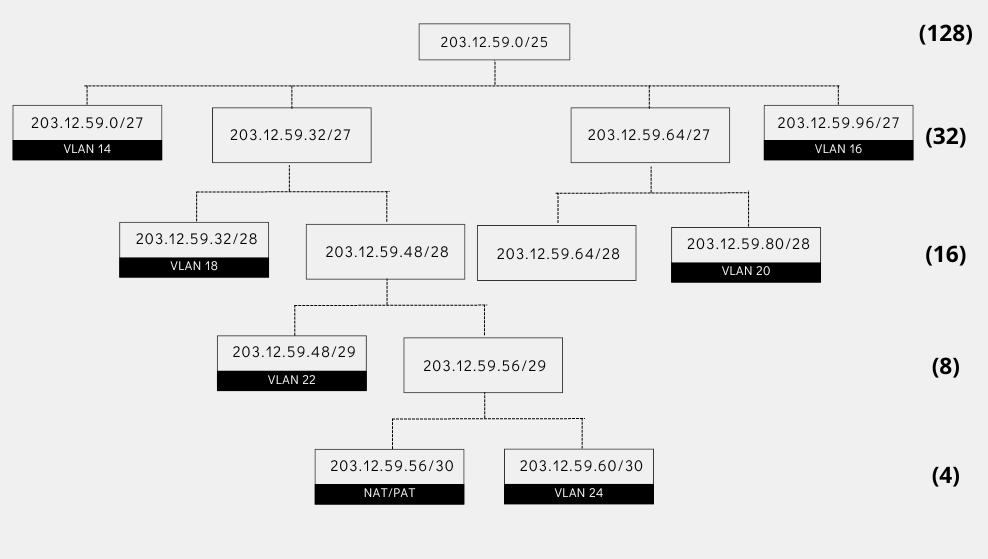
\includegraphics[width=18cm]{images/Horoscope Inc - IPv4 Publico.png}
   % \caption{Legenda da imagem, se desejar} % Opcional
\end{figure}

\newpage
\clearpage

\section*{\centerline{Private IPv4}}

\section*{Calendar Inc}

\begin{table}[h!]
\hspace*{-2.2cm}
\centering
%\begin{tabular}{|m{2cm}|m{1,3cm}|m{2,3cm}|m{5cm}|m{2,5cm}|m{1cm}|}
\begin{tabular}{|c|c|c|c|c|c|}
    \hline
    & \textbf{Máscara} & \textbf{Rede} & \textbf{Endereços Disponíveis} & \textbf{Broadcast} & \textbf{Default Gateway} \\ \hline
    VLAN2 & 24 & 172.26.12.0 & 172.26.12.2 a 172.26.12.254 & 172.26.12.255 & 172.26.12.1 \\ \hline
    VLAN4 & 25 & 172.26.13.128 & 172.26.13.130 a 172.26.13.254 & 172.26.13.255 & 172.26.13.129\\ \hline
    VLAN6 & 26 & 172.26.13.0 & 172.26.13.2 a 172.26.13.62 & 172.26.13.63 & 172.26.13.1\\ \hline
    VLAN8 & 27 & 172.26.13.96 & 172.26.13.98 a 172.26.13.126 & 172.26.13.127 & 172.26.13.97\\ \hline
    VLAN12 & --- & --- & --- & --- & --- \\ \hline
\end{tabular}
\caption{Atribuição do IPv4 Privado para Calendar Inc}
\label{tab:exemplo5x6}
\end{table}

\begin{figure}[H]
   \hspace*{-2.0cm}
    \centering
    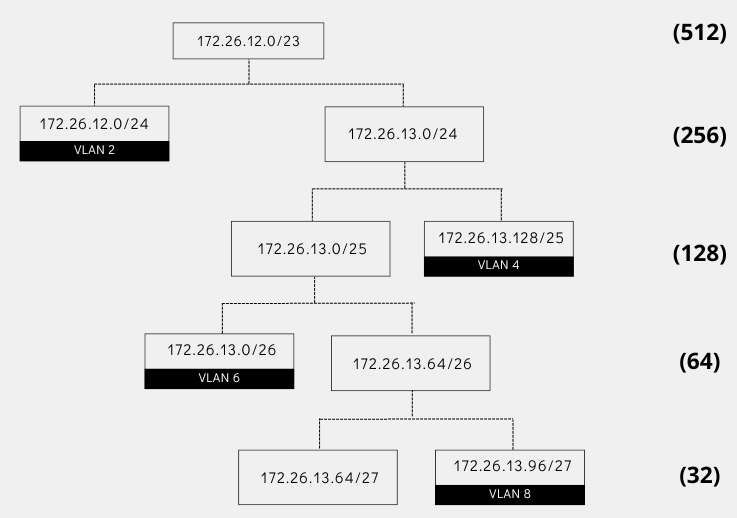
\includegraphics[width=16cm]{images/ipv4_priv_calendar.png}
   % \caption{Legenda da imagem, se desejar} % Opcional
\end{figure}

\newpage
\clearpage

\section*{Horoscope Inc}

\begin{table}[h!]
\hspace*{-2.0cm}
\centering
%\begin{tabular}{|m{2cm}|m{1,3cm}|m{2,3cm}|m{5cm}|m{2,5cm}|m{1cm}|}
\begin{tabular}{|c|c|c|c|c|c|}
    \hline
    & \textbf{Máscara} & \textbf{Rede} & \textbf{Endereços Disponíveis} & \textbf{Broadcast} & \textbf{Default Gateway} \\ \hline
    VLAN14 & 27 & 172.22.13.64 & 172.22.13.66 a 172.22.13.94 & 172.22.13.95 & 172.22.13.65 \\ \hline
    VLAN16 & 26 & 172.22.13.192 & 172.22.13.194 a 172.22.13.254 & 172.22.13.255 & 172.22.13.193 \\ \hline
    VLAN18 & 26 & 172.22.13.0 & 172.22.13.2 a 172.22.13.62 & 172.22.13.63 & 172.22.13.1 \\ \hline
    VLAN20 & 28 & 172.22.13.96 & 172.22.13.98 a 172.22.13.110 & 172.22.13.111 & 172.22.13.97 \\ \hline
    VLAN22 & 24 & 172.22.12.0 & 172.22.12.2 a 172.22.12.254 & 172.22.12.255 & 172.22.12.1 \\ \hline
    VLAN24 & --- & --- & --- & --- & --- \\ \hline
\end{tabular}
\caption{Atribuição do IPv4 Privado para Horoscope Inc}
\label{tab:exemplo5x6}
\end{table}

\begin{figure}[H]
    \hspace*{-2.0cm}
    \centering
    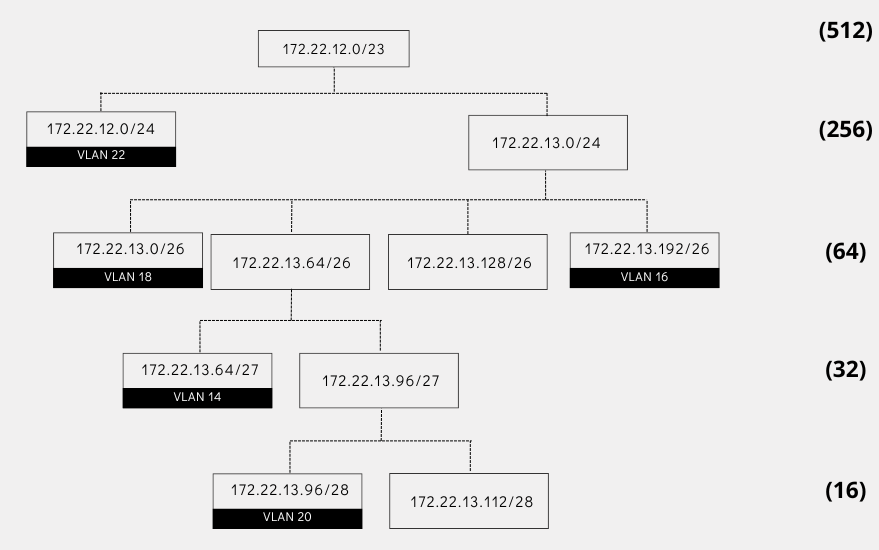
\includegraphics[width=16cm]{images/Horoscope Inc - IPv4 Privado.png}
   % \caption{Legenda da imagem, se desejar} % Opcional
\end{figure}

\newpage
\clearpage

\section*{\centerline{Global IPv6}}

\section*{Calendar Inc}

\begin{table}[h!]
    \hspace*{-4.0cm}
    \centering
    \setlength{\tabcolsep}{2pt} % Reduz o espaçamento entre colunas
    \renewcommand{\arraystretch}{1.3} % Aumenta o espaçamento entre linhas
    \begin{tabular}{|c|c|c|c|p{7.8cm}|} % Reduz a largura do campo Endereços Disponíveis
        \hline
        \textbf{Interface} & \textbf{Rede Interface} & \textbf{VLAN} & \textbf{Rede VLAN} & \textbf{Endereços Disponíveis} \\ \hline
        
        f1/1 (R2) & 2002:A198:BC26::/126 & --- & --- & --- \\ \hline
        
        f0/0 (ESW2) & 2002:A198:BC26::4/126 & --- & --- & --- \\ \hline
        
        \multirow{3.5}{*}{f2/1 (R2)} & \multirow{3.5}{*}{2002:A198:BC26:100::/56} & 6 & 2002:A198:BC26:106::/64 & 2002:A198:BC26:106::1/64 a 2002:A198:BC26:106:FFFF:FFFF:FFFF:FFFF/64 \\ \cline{3-5}   
         & & 8 & 2002:A198:BC26:108::/64 & 2002:A198:BC26:108::/64 a 2002:A198:BC26:108:FFFF:FFFF:FFFF:FFFF/64 \\ \cline{3-5} \hline
         
        \multirow{5}{*}{f1/14 (ESW2)} & \multirow{5}{*}{2002:A198:BC26:200::/56} & 2 & 2002:A198:BC26:202::/64 & 2002:A198:BC26:202::1/64 a 2002:A198:BC26:202:FFFF:FFFF:FFFF:FFFF/64 \\ \cline{3-5} 
         & & 4 & 2002:A198:BC26:204::/64 & 2002:A198:BC26:204::1/64 a 2002:A198:BC26:204:FFFF:FFFF:FFFF:FFFF/64 \\ \cline{3-5}   
         & & 12 & 2002:A198:BC26:20C::/64 & 2002:A198:BC26:20C::1/64 a 2002:A198:BC26:20C:FFFF:FFFF:FFFF:FFFF/64 \\ \hline
         
         \multirow{3.5}{*}{f1/15 (ESW2)} & \multirow{3.5}{*}{2002:A198:BC26:300::/56} & 2 & 2002:A198:BC26:302::/64 & 2002:A198:BC26:302::1/64 a 2002:A198:BC26:302:FFFF:FFFF:FFFF:FFFF/64 \\ \cline{3-5}   
         & & 4 & 2002:A198:BC26:304::/64 & 2002:A198:BC26:304::1/64 a 2002:A198:BC26:304:FFFF:FFFF:FFFF:FFFF/64 \\ \cline{3-5} \hline

    \end{tabular}
    \caption{Atribuição do IPv6 Global para Calendar Inc}
\end{table}


\begin{figure}[H]
    %\hspace*{-1.0cm}
    \centering
    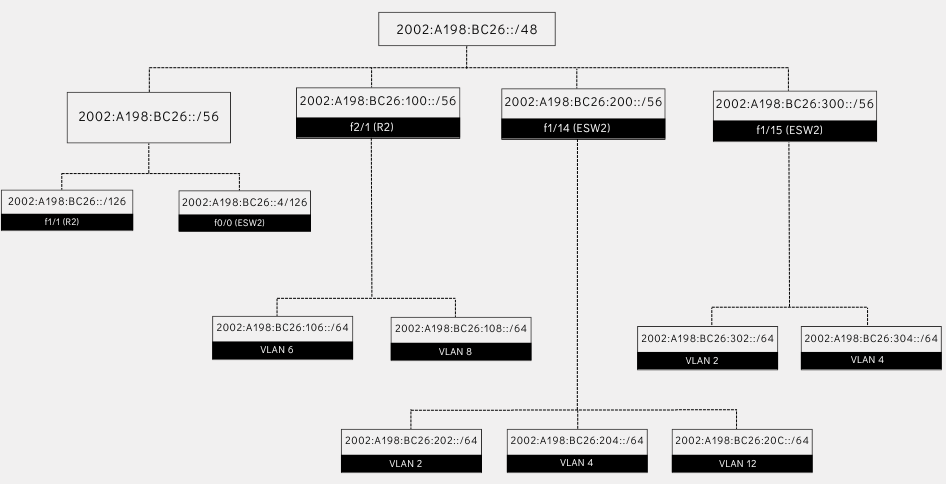
\includegraphics[width=12cm]{images/ipv6_global_calendar.png}
   % \caption{Legenda da imagem, se desejar} % Opcional
\end{figure}

\newpage
\clearpage

\section*{Horoscope Inc}

%\begin{tabular}{|m{2cm}|m{1,3cm}|m{2,3cm}|m{5cm}|m{2,5cm}|m{1cm}|}

\begin{table}[h!]
    \hspace*{-4.0cm}
    \centering
    \setlength{\tabcolsep}{2pt} % Reduz o espaçamento entre colunas
    \renewcommand{\arraystretch}{1.3} % Aumenta o espaçamento entre linhas
    \begin{tabular}{|c|c|c|c|p{7.8cm}|} % Reduz a largura do campo Endereços Disponíveis
        \hline
        \textbf{Interface} & \textbf{Rede Interface} & \textbf{VLAN} & \textbf{Rede VLAN} & \textbf{Endereços Disponíveis} \\ \hline

        f1/0 (R1) & 2002:A125:BC91::/126 & --- & --- & --- \\ \hline
        
        f0/0 (ESW1) & 2002:A125:BC91::4/126 & --- & --- & --- \\ \hline
        
        \multirow{5}{*}{f2/0 (R1)} & \multirow{5}{*}{2002:A125:BC91:100::/56} & 14 & 2002:A125:BC91:10E::/64 & 2002:A125:BC91:10E::1/64 a 2002:A125:BC91:10E:FFFF:FFFF:FFFF:FFFF/64 \\ \cline{3-5} 
         & & 16 & 2002:A125:BC91:110::/64 & 2002:A125:BC91:110::1/64 a 2002:A125:BC91:110:FFFF:FFFF:FFFF:FFFF/64 \\ \cline{3-5}   
         & & 24 & 2002:A125:BC91:118::/64 & 2002:A125:BC91:118::1/64 a 2002:A125:BC91:118:FFFF:FFFF:FFFF:FFFF/64 \\ \hline
         
         \multirow{5}{*}{f1/13 (ESW1)} & \multirow{5}{*}{2002:A125:BC91:200::/56} & 18 & 2002:A125:BC91:212::/64 & 2002:A125:BC91:212::1/64 a 2002:A125:BC91:212:FFFF:FFFF:FFFF:FFFF/64 \\ \cline{3-5}   
         & & 20 & 2002:A125:BC91:214::/64 & 2002:A125:BC91:214::1/64 a 2002:A125:BC91:214:FFFF:FFFF:FFFF:FFFF/64 \\ \cline{3-5}   
         & & 22 & 2002:A125:BC91:216::/64 & 2002:A125:BC91:216::1/64 a 2002:A125:BC91:216:FFFF:FFFF:FFFF:FFFF/64 \\ \hline
        
        f1/14 (ESW1) & 2002:A125:BC91:300::/56 & 20 & 2002:A125:BC91:314::/64 & 2002:A125:BC91:314::1/64 a 2002:A125:BC91:314:FFFF:FFFF:FFFF:FFFF/64 \\ \hline
        
        f1/15 (ESW1) & 2002:A125:BC91:400::/56 & 18 & 2002:A125:BC91:412::/64 & 2002:A125:BC91:412::1/64 a 2002:A125:BC91:412:FFFF:FFFF:FFFF:FFFF/64 \\ \hline

    \end{tabular}
    \caption{Atribuição do IPv6 Global para Horoscope Inc}
\end{table}



\begin{figure}[H]
    %\hspace*{-1.0cm}
    \centering
    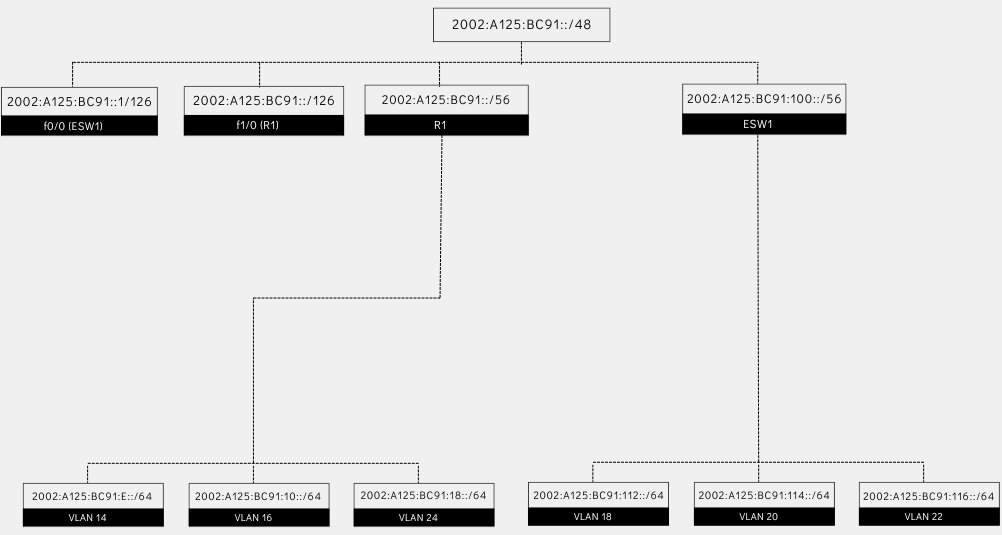
\includegraphics[width=12.5cm]{images/Horoscope Inc - IPv6.png}
   % \caption{Legenda da imagem, se desejar} % Opcional
\end{figure}

%%%%%%%%%%%%%%%%%%%%%%%%%%%%%%%%%
\printbibliography

\end{document}